%=====================================================================
%  Theory seminar:  Light-cone perturbation theory and the soft gluon
%  wave function / evolution operator in the CGC at NLO
%  Based on: R. Radhakrishnan, arXiv:2607.18373
%  Audience: QCD experts, no small-x background.  Length: 30-40 min.
%=====================================================================
\documentclass[9pt,aspectratio=169]{beamer}

\usetheme[progressbar=frametitle,numbering=fraction,block=fill]{metropolis}
\usepackage{appendixnumberbeamer}
\usepackage{amsmath,amssymb,bm}
\usepackage{tikz}
\usetikzlibrary{decorations.pathmorphing,arrows.meta,positioning,calc,patterns}
\usepackage{booktabs}

% ---- colours -------------------------------------------------------
\definecolor{acc}{HTML}{C1272D}       % accent / highlight
\definecolor{blu}{HTML}{1F4E79}       % structure
\definecolor{grn}{HTML}{1B7A3D}
\definecolor{gry}{HTML}{6E7377}
\setbeamercolor{alerted text}{fg=acc}
\setbeamercolor{frametitle}{bg=blu}
\setbeamercolor{progress bar}{fg=acc}
\setbeamercolor{title separator}{fg=acc}

\newcommand{\hl}[1]{\textcolor{acc}{#1}}
\newcommand{\hb}[1]{\textcolor{blu}{#1}}
\newcommand{\hg}[1]{\textcolor{grn}{#1}}

% ---- macros --------------------------------------------------------
\newcommand{\pp}{p^{+}}
\newcommand{\kp}{k^{+}}
\newcommand{\xm}{x^{-}}
\newcommand{\xp}{x^{+}}
\newcommand{\dthree}[1]{\frac{d^{3}#1}{(2\pi)^{3}}}
\newcommand{\Om}{\Omega}
\newcommand{\Qs}{Q_{s}}
\newcommand{\ket}[1]{\left|#1\right\rangle}
\newcommand{\bra}[1]{\left\langle#1\right|}
\newcommand{\bk}[2]{\left\langle#1\middle|#2\right\rangle}
\newcommand{\Hg}{H_{g}}
\newcommand{\Hggg}{H_{ggg}}
\newcommand{\ad}{a^{\dagger}}
\newcommand{\WW}{\text{WW}}

% ---- tikz styles ---------------------------------------------------
\tikzset{
  gluon/.style={decorate, decoration={coil,aspect=0,segment length=5pt,amplitude=2.6pt}, thick, blu},
  val/.style={very thick, black},
  cut/.style={dashed, gray, thin},
  blob/.style={circle, fill=acc, inner sep=1.6pt},
}

% ---- title ---------------------------------------------------------
\title{Light-Cone Perturbation Theory and the Soft Gluon Wave Function}
\subtitle{The CGC evolution operator $\Omega$ at next-to-leading order}
\date{Theory Seminar \quad\textbullet\quad \today}
\author{\textit{[speaker]}}
\institute{based on \textbf{R.~Radhakrishnan}, \texttt{arXiv:2607.18373} (JHEP submission)}

\begin{document}

\maketitle

%=====================================================================
\begin{frame}{Where we are going}
\begin{columns}[T,onlytextwidth]
\column{0.5\textwidth}
\textbf{Part I --- Light-front dynamics}\\[2pt]
{\small Quantisation on $\xp=$ const; why the vacuum is trivial;
light-cone gauge; \hl{LCPT} = old-fashioned perturbation theory done right.}
\medskip

\textbf{Part II --- Why small-$x$ people care}\\[2pt]
{\small Saturation in 10 minutes for a QCD expert: classical sources,
Wilson lines, and why the \hl{projectile wave function} is the object we need.}

\column{0.5\textwidth}
\textbf{Part III --- The paper}\\[2pt]
{\small Construct the unitary boost operator $\Om$ with
$\ket{\Psi_n}=\Om\ket{n}$ to $\mathcal{O}(g^2)$ in pure Yang--Mills:
\begin{itemize}\small
  \item normal-ordered ansatz with \hl{operator-valued} coefficients,
  \item fixed by \hl{unitarity} $+$ \hl{matching to LCPT},
  \item application: $\Om^\dagger H\,\Om$ is diagonal through $\mathcal{O}(g^2)$.
\end{itemize}}
\end{columns}
\vfill
\begin{alertblock}{One-sentence summary}
$\Om$ is the operator that dresses a fast hadron with its soft gluon cloud ---
at leading order it is a coherent state, and \hl{everything interesting starts
at the next order}.
\end{alertblock}
\end{frame}

%=====================================================================
\section{Part I --- Light-front dynamics and LCPT}
%=====================================================================

\begin{frame}{Dirac's forms of relativistic dynamics}
Choose a foliation of spacetime; the generators of the Poincar\'e group split into
\hb{kinematical} (preserve the surface) and \hl{dynamical} (evolve it).
\medskip
\begin{center}
\small
\begin{tabular}{lccl}
\toprule
Form & surface & \# kinematical & Hamiltonian\\
\midrule
Instant & $t=0$ & 6 & $P^{0}$\\
\hl{Front} & $\xp=(t+z)/\sqrt2=0$ & \hl{7} & $P^{-}$\\
Point & $x^\mu x_\mu = a^2$ & 6 & \\
\bottomrule
\end{tabular}
\end{center}
\medskip
The front form is the \hl{maximally kinematical} one. In particular:
\begin{itemize}
  \item \hb{Boosts along $z$ are kinematical}: $p^{+}\!\to e^{\omega}p^{+}$, $\bm{p}$ untouched.
        A light-front wave function does \emph{not} change shape under a longitudinal boost.
  \item Transverse boosts act as \emph{Galilean} transformations in the $(\bm p, p^+)$ plane.
\end{itemize}
\medskip
\begin{block}{Why a high-energy physicist should care}
Collider physics is about states boosted to enormous rapidity. In the front form
the boost is trivial, and \hl{parton distributions / LCWFs are frame-independent objects}.
\end{block}
\end{frame}

%=====================================================================
\begin{frame}{Conventions}
\[
x^{\pm}=\tfrac{1}{\sqrt2}\,(x^{0}\pm x^{3}),\qquad
x^{\mu}=(\xp,\xm,\bm x),\qquad
p\cdot x = \pp \xm + p^{-}\xp - \bm p\!\cdot\!\bm x .
\]
\vspace{-6pt}
\begin{columns}[T,onlytextwidth]
\column{0.58\textwidth}
\begin{itemize}
  \item $\xp$ = \hl{light-cone time}; quantise on $\xp=$ const.
  \item $p^{-}$ = \hl{light-cone energy}, generates $\xp$ translations $\Rightarrow$ the Hamiltonian.
  \item $\pp$ = longitudinal momentum, \hb{conserved and positive}.
  \item Measure $d^{3}p \equiv d\pp\, d^{2}\bm p$, \;
        $\delta^{3}(k-p)\equiv\delta(\kp-\pp)\delta^{(2)}(\bm k-\bm p)$.
\end{itemize}
\column{0.40\textwidth}
\vspace{-10pt}
\begin{center}
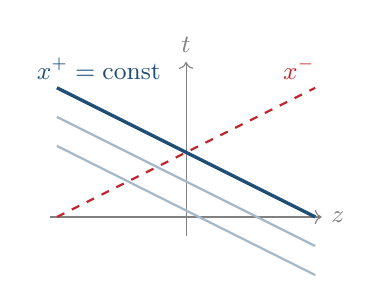
\begin{tikzpicture}[scale=0.82]
  \draw[->,gray] (-2.1,0)--(2.1,0) node[right]{\small $z$};
  \draw[->,gray] (0,-0.3)--(0,2.4) node[above]{\small $t$};
  \foreach \s in {0.0,0.45,0.9} {
    \draw[blu!40,thick] (-2.0,2.0-\s)--(2.0,-0.0-\s);}
  \draw[very thick,blu] (-2.0,2.0)--(2.0,0.0);
  \draw[dashed,acc,thick] (-2.0,-0.0)--(2.0,2.0);
  \node[blu] at (-1.35,2.3) {\small $\xp=\text{const}$};
  \node[acc] at (1.75,2.3) {\small $\xm$};
\end{tikzpicture}
\end{center}
\end{columns}
\vspace{-2pt}
\begin{alertblock}{On shell ($m=0$)}
\vspace{-10pt}
\[
p^{-}=\frac{\bm p^{2}}{2\pp}
\]
\vspace{-12pt}
\begin{center}
Non-relativistic in form: $\pp$ plays the role of a mass, $\bm p$ of a 2D momentum,
$p^{-}$ of the kinetic energy.
\end{center}
\end{alertblock}
\end{frame}

%=====================================================================
\begin{frame}{The one property that makes everything work}
\begin{alertblock}{Positivity of $\pp$ $\Rightarrow$ trivial vacuum}
For any physical quantum $\pp>0$, and $\pp$ is \emph{conserved} at every vertex.
A state with $P^{+}=0$ cannot fluctuate into anything with particles in it.
\[
\ket{0}_{\text{free}} \;=\; \ket{0}_{\text{interacting}} \qquad\text{(perturbatively)}
\]
\end{alertblock}
\medskip
Contrast with the equal-time formulation, where the vacuum is a complicated
condensate of $q\bar q$ and $gg$ pairs and the Fock expansion of a hadron is
\emph{not} meaningful.
\medskip
\begin{block}{Consequence: the Fock expansion is physical}
\[
\ket{\Psi_{h}} = \psi_{0}\ket{0} + \psi_{g}\ket{g} + \psi_{gg}\ket{gg}+\psi_{ggg}\ket{ggg}+\cdots
\]
with $|\psi_{n}|^{2}$ a genuine \hl{probability} to find that configuration in the hadron.
\end{block}
\medskip
{\small (The price: zero modes $\pp\!\to\!0$ hide the non-trivial QCD vacuum ---
chiral symmetry breaking, $\theta$-vacuum. Not our problem today: we work with
an explicit IR cutoff $\Lambda$ on $\pp$.)}
\end{frame}

%=====================================================================
\begin{frame}{Light-cone gauge $A^{+}=0$}
\begin{itemize}
  \item Only $A^{i}$, $i=1,2$ remain \hl{dynamical}: two physical polarisations, \hb{no ghosts}.
  \item $A^{-}$ is a \hl{constrained} field --- solved from the $+$ component of the EOM,
  \[
    \partial^{+}A^{a}_{+} = -\frac{1}{\partial^{+}}\!\left(D^{ab}_{i}\partial^{+}A^{b}_{i}-gJ^{a+}\right),
  \]
  and eliminated from the Hamiltonian.
  \item The price: \hl{non-local $1/\partial^{+}$ kernels} $\to$ \hb{instantaneous} interactions
  (light-front analogue of the Coulomb term in $A^{0}=0$ gauge).
\end{itemize}
\vspace{-2pt}
\begin{block}{Pure Yang--Mills LC Hamiltonian ($N_{f}=0$)}
\[
H^{LC}_{\rm YM}=\int\! d\xm d^{2}\bm x\;
\Big[\tfrac12 \Pi^{a}\Pi^{a}+\tfrac14 F^{a}_{ij}F^{a}_{ij}\Big],
\quad
\Pi^{a}\equiv -\tfrac{1}{\partial^{+}}\big(D^{ab}_{i}\partial^{+}A^{b}_{i}\big)
\]
\end{block}
\begin{align*}
H_{\rm int}=\int\! d\xm d^{2}\bm x\Big[&
\underbrace{-gf^{abc}A^{b}_{i}A^{c}_{j}\partial_{i}A^{a}_{j}}_{3g\ \text{vertex}}
\;+\;\underbrace{\tfrac{g^{2}}{4}f^{abc}f^{ade}A^{b}_{i}A^{c}_{j}A^{d}_{i}A^{e}_{j}}_{4g\ \text{vertex}}\\[-2pt]
&\underbrace{-gf^{abc}(\partial_iA^a_i)\tfrac{1}{\partial^+}\big(A^b_j\partial^+A^c_j\big)
\;+\;\tfrac{g^{2}}{2}f^{abc}f^{ade}\tfrac{1}{\partial^{+}}\big(A^{b}_{i}\partial^{+}\!A^{c}_{i}\big)
\tfrac{1}{\partial^{+}}\big(A^{d}_{j}\partial^{+}\!A^{e}_{j}\big)}_{\hl{\text{instantaneous}}}\Big]
\end{align*}
\end{frame}

%=====================================================================
\begin{frame}{Light-cone perturbation theory (LCPT)}
LCPT $=$ \hl{old-fashioned (time-ordered) perturbation theory} on null planes.
Split $H=H_{0}+H_{\rm int}$ and solve $H\ket{\Psi}=E\ket{\Psi}$ perturbatively:
\[
\ket{\Psi^{(1)}_{n}}=\sum_{m\neq n}\ket{m}\frac{\bra{m}H_{\rm int}\ket{n}}{E_{n}-E_{m}},
\qquad E_{n}=\sum_{i\in n}\frac{\bm k_{i}^{2}}{2k^{+}_{i}} .
\]
\begin{columns}[T,onlytextwidth]
\column{0.53\textwidth}
\textbf{Rules}
\begin{enumerate}\small
  \item Draw all \hl{$\xp$-orderings} of a graph.
  \item $(\pp,\bm p)$ conserved at each vertex; \hb{$p^{-}$ is not}.
  \item Every intermediate state: all lines \hl{on shell}, all $\pp>0$.
  \item One \hl{energy denominator} $\big(E_{\rm in}-E_{\rm interm.}\big)^{-1}$ per intermediate state.
  \item Add the \hl{instantaneous} vertices.
\end{enumerate}
\vspace{-4pt}
\column{0.45\textwidth}
\textbf{Relation to covariant diagrams}\\[2pt]
{\small Do the $k^{-}$ contour integral of a Feynman diagram by residues:
\[
\text{1 covariant graph}=\!\!\sum_{\substack{\xp\text{-orderings}\\ \text{with all }\pp>0}}\!\!\text{LCPT graphs}
\]
Orderings with a negative $\pp$ line collapse to the \hl{instantaneous} pieces.
Many orderings vanish $\Rightarrow$ fewer terms than naive OFPT.}
\end{columns}
\vspace{-6pt}
{\small\hl{Why use it here:} each term is a \emph{physical intermediate state} with a
probabilistic reading --- exactly what you need when the observable \emph{is} a wave function.}
\end{frame}

%=====================================================================
\begin{frame}{LCPT in one picture}
\begin{center}
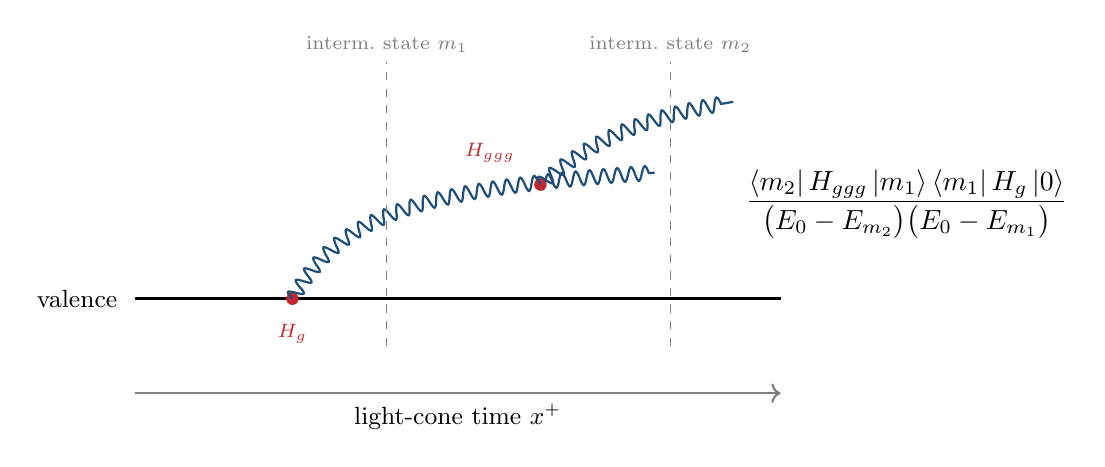
\begin{tikzpicture}[scale=1.0]
  % valence line
  \draw[val] (-4.6,0)--(3.6,0);
  \node[left] at (-4.7,0) {\small valence};
  % emission 1
  \coordinate (v1) at (-2.6,0);
  \coordinate (v2) at (-0.2,0);
  \node[blob] at (v1) {};
  \draw[gluon] (v1) .. controls (-2.0,1.0) and (-1.2,1.4) .. (2.0,1.6);
  % splitting
  \coordinate (s) at (0.55,1.42);
  \node[blob] at (0.55,1.45) {};
  \draw[gluon] (0.55,1.45) .. controls (1.2,2.0) and (1.8,2.3) .. (3.0,2.5);
  % cuts
  \draw[cut] (-1.4,-0.6)--(-1.4,3.0);
  \draw[cut] ( 2.2,-0.6)--( 2.2,3.0);
  \node[gray,above] at (-1.4,3.0) {\scriptsize interm.\ state $m_1$};
  \node[gray,above] at ( 2.2,3.0) {\scriptsize interm.\ state $m_2$};
  \node[acc,below] at (-2.6,-0.2) {\scriptsize $\Hg$};
  \node[acc,left] at (0.35,1.85) {\scriptsize $\Hggg$};
  \node at (5.2,1.2) {$\displaystyle \frac{\bra{m_2}H_{ggg}\ket{m_1}\bra{m_1}H_{g}\ket{0}}{\big(E_0-E_{m_2}\big)\big(E_0-E_{m_1}\big)}$};
  \draw[->,gray,thick] (-4.6,-1.2)--(3.6,-1.2) node[midway,below,black]{\small light-cone time $\xp$};
\end{tikzpicture}
\end{center}
\medskip
\begin{itemize}
  \item Dashed lines $=$ where we ``cut'' and evaluate $E_{\rm in}-E_{\rm interm.}$.
  \item Each vertex is a matrix element of $H_{\rm int}$ between \emph{on-shell} Fock states.
  \item \hl{Everything today is built out of exactly this object.}
\end{itemize}
\end{frame}

%=====================================================================
\section{Part II --- Small-$x$ and the CGC in ten minutes}
%=====================================================================

\begin{frame}{The small-$x$ problem, stated for a QCD expert}
\begin{columns}[T,onlytextwidth]
\column{0.55\textwidth}
\begin{itemize}
  \item DGLAP/BFKL: the gluon density grows fast, $xG(x,Q^{2})\sim x^{-\lambda}$, $\lambda\approx0.3$.
  \item Occupation number of a mode $\bm k$ in a hadron of area $S_\perp$:
  \[
     n(\bm k)\sim \frac{\alpha_{s}}{\bm k^{2}}\frac{xG(x,Q^2)}{S_{\perp}}
  \]
  \item Linear evolution $\Rightarrow n\sim 1/\alpha_{s}$: \hl{fields are classically strong},
        $A_\mu\sim1/g$. Recombination $gg\to g$ can no longer be neglected.
  \item Balance defines the \hl{saturation scale}
  \[
      \Qs^{2}(x)\;\sim\;\alpha_{s}\frac{xG(x,\Qs^{2})}{S_{\perp}}\;\gg\;\Lambda^{2}_{\rm QCD}.
  \]
\end{itemize}
\column{0.43\textwidth}
\begin{center}
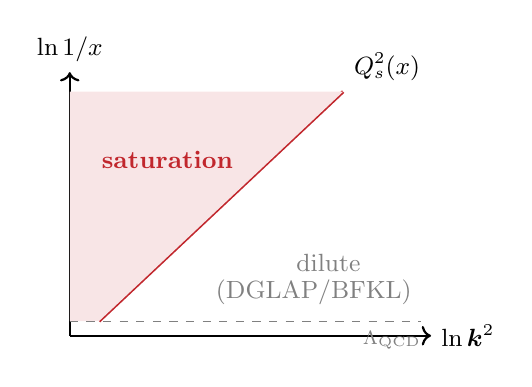
\begin{tikzpicture}[scale=0.62]
  \draw[->,thick] (0,0)--(7.4,0) node[right]{\small $\ln \bm k^2$};
  \draw[->,thick] (0,0)--(0,5.4) node[above]{\small $\ln 1/x$};
  \draw[very thick,acc] (0.6,0.3)--(5.6,5.0) node[above right,black]{\small $\Qs^{2}(x)$};
  \fill[acc!12] (0.6,0.3)--(5.6,5.0)--(0,5.0)--(0,0.3)--cycle;
  \node[acc] at (2.0,3.6) {\small \textbf{saturation}};
  \node[gray] at (5.3,1.5) {\small dilute};
  \node[gray] at (5.0,0.9) {\small (DGLAP/BFKL)};
  \draw[dashed,gray] (0,0.3)--(7.2,0.3);
  \node[gray,below] at (6.6,0.3) {\scriptsize $\Lambda_{\rm QCD}$};
\end{tikzpicture}
\end{center}
\end{columns}
\medskip
\begin{alertblock}{The effective theory}
Colour Glass Condensate: separate the hadron by longitudinal momentum ---
\hl{fast partons} $=$ frozen colour sources $\rho$, \hl{slow gluons} $=$ the field they radiate.
\end{alertblock}
\end{frame}

%=====================================================================
\begin{frame}{CGC: sources $+$ field, and the Born--Oppenheimer logic}
\begin{columns}[T,onlytextwidth]
\column{0.56\textwidth}
Split the gauge field by longitudinal momentum,
\[
A^{a}_{i}=\underbrace{\bar{\mathcal A}^{a}_{i}}_{\kp\ \ge\ \vee\ \text{(valence)}}
\;+\;\underbrace{A^{a}_{i}}_{\Lambda<\kp<\vee\ \text{(soft)}} .
\]
\begin{itemize}
  \item Valence modes have much larger $\kp$ $\Rightarrow$ much \hl{longer} LC time dilation:
        they are \hb{static} on the soft time scale.
  \item Born--Oppenheimer: soft gluons see the valence sector only through its
        \hl{colour charge density}
  \[
   \rho^{a}(-\bm p)=-if^{abc}\!\!\int_{\vee}^{\infty}\!\!\frac{d\kp}{2\pi}\frac{d^2\bm k}{(2\pi)^2}
   \ad{}^{b}_{j}(k)a^{c}_{j}(k+p).
  \]
\end{itemize}
\column{0.43\textwidth}
\begin{center}
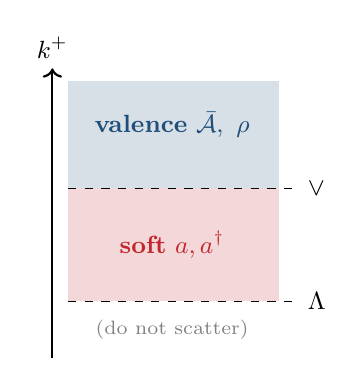
\begin{tikzpicture}[scale=0.8]
 \draw[->,thick] (0,-0.2)--(0,4.4) node[above]{\small $\kp$};
 \fill[blu!18] (0.25,2.5) rectangle (3.6,4.2);
 \fill[acc!18] (0.25,0.7) rectangle (3.6,2.5);
 \node[blu] at (1.9,3.5) {\small \textbf{valence} $\bar{\mathcal A},\ \rho$};
 \node[acc] at (1.9,1.6) {\small \textbf{soft} $a,\ad$};
 \draw[dashed] (0.25,2.5)--(3.9,2.5) node[right,black]{\small $\vee$};
 \draw[dashed] (0.25,0.7)--(3.9,0.7) node[right,black]{\small $\Lambda$};
 \node[gray] at (1.9,0.25) {\scriptsize (do not scatter)};
\end{tikzpicture}
\end{center}
\end{columns}
\medskip
\begin{alertblock}{The crucial non-Abelian twist}
$\rho$ is an \hl{operator}, not a c-number:
$\;[\rho^{a}(\bm k),\rho^{b}(\bm p)]=if^{abc}\rho^{c}(\bm k+\bm p)$.\\
Every coefficient below is a functional of $\rho$ $\Rightarrow$ \hb{ordering matters everywhere}.
\end{alertblock}
\end{frame}

%=====================================================================
\begin{frame}{The eikonal approximation and the soft Hamiltonian}
\hl{Eikonal:} drop everything suppressed by $\kp_{\rm soft}/\kp_{\rm valence}$.
Operationally, $\tfrac{1}{\partial^{+}}$ acting on a \emph{valence} field is dropped,
$\;\tfrac{1}{\partial^{+}}\!\big(A^{b}_{j}\partial^{+}\bar{\mathcal A}^{c}_{j}\big)\simeq 0$.
\medskip

After mode decomposition the interaction organises as
\[
H_{\rm int}=\hl{\Hg}+\hl{\Hggg}+H_{gggg}+H_{gg\text{-inst}}+H_{gggg\text{-inst}}+H_{V}.
\]
\begin{block}{The key vertex: soft gluon emission off the source ($\mathcal{O}(g)$, one $\rho$)}
\[
\Hg=\int_{\Lambda}^{\vee}\!\frac{d\kp}{2\pi}\frac{d^{2}\bm k}{(2\pi)^{2}}\;
\frac{g\,k_{i}}{\sqrt2\,|\kp|^{3/2}}
\Big[\ad{}^{a}_{i}(k)\rho^{a}(-\bm k)+a^{a}_{i}(k)\rho^{a}(\bm k)\Big]
\]
\end{block}
\begin{itemize}
  \item $\Hggg$ --- the genuine non-Abelian $3g$ vertex among \emph{soft} gluons; \hl{$\rho$-independent}.
  \item $H_{gg\text{-inst}}$ --- valence instantaneously makes/absorbs a soft pair.
  \item $H_{V}$ --- valence-only; decouples from the soft dynamics.
\end{itemize}
\medskip
{\small Note the two \hb{independent} labels: (\# soft gluons $n$, \# of $\rho$ insertions $m$).
A given order in $g$ mixes different $m$.}
\end{frame}

%=====================================================================
\begin{frame}{What physics actually needs the wave function}
\begin{block}{Single inclusive gluon production at mid-rapidity}
\[
\frac{dN}{d^{2}\bm k\,dy}\;\propto\;
\big\langle \Psi_{\rm proj}\big|\;\hat{S}^{\dagger}\,\ad_{i}(k)a_{i}(k)\,\hat S\;\big|\Psi_{\rm proj}\big\rangle
\]
\begin{itemize}
  \item $\ket{\Psi_{\rm proj}}=\Om\ket{v}$: the projectile \hl{boosted} by $\Om$.
  \item $\hat S$: eikonal scattering off the target field $\Rightarrow$ \hb{Wilson lines}
        $a\to V^{ab}a^{b}$, $V=\mathcal{P}\exp\!\big[ig\!\int\! d\xm A^{-}_{\rm tgt}\big]$.
  \item Average over the valence configurations $\rho$ with the CGC weight.
\end{itemize}
\end{block}
\vspace{-2pt}
So the calculation factorises into three ingredients, and \hl{only one of them is hard}:
\begin{center}
\scriptsize
\begin{tabular}{lll}
\toprule
ingredient & status at LO & status at NLO\\
\midrule
target Wilson lines & known & known (BK/JIMWLK)\\
eikonal $\hat S$ & known & known\\
\hl{projectile wave function $\Om$} & coherent state & \hl{this talk}\\
\bottomrule
\end{tabular}
\end{center}
\vspace{-2pt}
{\small Same $\Om$ also generates the \hl{JIMWLK} Hamiltonian when the soft modes are
integrated out --- its $\mathcal{O}(g^{2})$ pieces feed NLO JIMWLK [Lublinsky--Mulian '17].}
\end{frame}

%=====================================================================
\section{Part III --- Constructing $\Omega$ at $\mathcal{O}(g^2)$}
%=====================================================================

\begin{frame}{The evolution operator $\Omega$: two equivalent definitions}
\begin{columns}[T,onlytextwidth]
\column{0.49\textwidth}
\textbf{(1) Dressing operator}
\[
\ket{\Psi_{n}}=\Om\ket{n},\qquad \Om=U(-\infty,0)
\]
{\small Adiabatically switch on $H_{\rm int}$: the free Fock state $\ket n$ evolves into
the corresponding eigenstate of the full $H$. Physically, $\Om$ \hl{is the boost}
by one rapidity slice: it fills the newly opened longitudinal phase space with soft gluons.}

\column{0.49\textwidth}
\textbf{(2) Diagonalising operator}
\[
\Om^{\dagger}H\,\Om=\sum_{n}E_{n}\ket{n}\bra{n}
\]
{\small Immediate from (1): $H\Om\ket n=E_n\Om\ket n$. So $\Om$ is chosen to kill the
off-diagonal matrix elements of $H$ between Fock sectors, order by order.}
\end{columns}
\medskip
\begin{alertblock}{Leading order: the coherent operator}
Only $\Hg$ survives $\;\Rightarrow$
\[
\Om\;\to\;C=\exp\!\int\!\dthree{p}\Big[\mathcal{A}^{b}_{j}(p)\ad{}^{b}_{j}(p)-\mathcal{A}^{\dagger b}_{j}(p)a^{b}_{j}(p)\Big],
\qquad
\mathcal{A}^{b}_{j}(p)=-\frac{\sqrt2\,g\,p_{j}\,\rho^{b}(-\bm p)}{\sqrt{\pp}\;\bm p^{2}}
\]
i.e.\ the \hl{Weizs\"acker--Williams} field of the valence charge. $C\ket0$ is a
\hb{coherent state}: independently emitted WW gluons.
\end{alertblock}
\end{frame}

%=====================================================================
\begin{frame}{Why leading order is not enough}
\begin{block}{At fixed $\rho$, a coherent state has no connected correlations}
\[
\langle \hat n(\bm k_1)\hat n(\bm k_2)\rangle_{\rho}
=\langle \hat n(\bm k_1)\rangle_{\rho}\,\langle \hat n(\bm k_2)\rangle_{\rho}
\]
Every multi-gluon observable \hl{factorises}.
All LO correlations (double-inclusive, the near-side ridge) come \emph{only}
from the subsequent \hb{averaging over $\rho$}.
\end{block}
\medskip
Beyond LO, the normal-ordered expansion of $\Om$ develops coefficients that are
\hl{genuinely connected multi-gluon emission amplitudes, present already before
averaging over $\rho$}. They contribute to
\begin{itemize}
  \item multiplicity \hb{fluctuations} (moments of $\hat N$ at $\mathcal{O}(g^{4})$),
  \item \hb{double-inclusive azimuthal correlations} and the near-side ridge,
  \item \hb{NLO single-inclusive} gluon production.
\end{itemize}
\medskip
\begin{alertblock}{Goal of the paper}
Determine \hl{all} coefficients of the normal-ordered $\Om$ through $\mathcal{O}(g^{2})$
in pure Yang--Mills, completing partial results of Lublinsky--Mulian '17.
\end{alertblock}
\end{frame}

%=====================================================================
\begin{frame}{Step 1: the most general normal-ordered ansatz}
Write $\Om$ fully normal ordered in the soft $a,\ad$, keeping every structure that can
contribute through $\mathcal{O}(g^{2})$:
\small
\begin{align*}
\Om=\;& N
 +\int_{p}\Big[\mathcal{A}_{1}a+\mathcal{A}_{2}\ad\Big]
 +\int_{p,q}\Big[B_{1}\,aa+B_{2}\,\ad\ad+B_{3}\,\ad a\Big]\\
 &+\int_{p,q,r}\Big[C_{1}\,\ad\ad a + C_{2}\,\ad a a\Big]
  +\int_{p,q,r,s}\Big[D_{1}\,\ad\ad\ad a + D_{2}\,\ad\ad a a + D_{3}\,\ad a a a\Big]\\
 &+\int_{p,\dots,v}\Big[E_{1}\,\ad\ad\ad\ad a a + E_{2}\,\ad\ad\ad a a a + E_{3}\,\ad\ad a a a a\Big]
\end{align*}
\normalsize
(colour, polarisation and momentum labels suppressed; $\int_p\equiv\int\! d^3p/(2\pi)^3$.)
\medskip
\begin{columns}[T,onlytextwidth]
\column{0.5\textwidth}
\begin{itemize}
  \item $\mathcal{A},\,C$ are $\mathcal{O}(g)$;
  \item $N-1,\;B,\;D,\;E$ are $\mathcal{O}(g^{2})$;
  \item all coefficients are \hl{operators} built from $\rho$ --- they do not commute.
\end{itemize}
\column{0.5\textwidth}
\begin{block}{Reading the structures}
$\ad$: real emission. $a$: absorption.\\
$\ad a$: propagation through the background.\\
$\ad\ad a$: $1\!\to\!2$ splitting of an existing gluon.
\end{block}
\end{columns}
\end{frame}

%=====================================================================
\begin{frame}{Step 2: two complementary sets of conditions}
\begin{columns}[T,onlytextwidth]
\column{0.49\textwidth}
\begin{block}{(a) Unitarity $\Om^{\dagger}\Om=1$}
Write $\Om=1+g\Om^{(1)}+g^{2}\Om^{(2)}+\dots$
\[
\mathcal{O}(g):\quad \Om^{(1)\dagger}=-\Om^{(1)}
\]
\[
\mathcal{O}(g^{2}):\quad \Om^{(2)}+\Om^{(2)\dagger}=-\Om^{(1)\dagger}\Om^{(1)}
\]
{\small Fixes precisely the pieces that matching \emph{cannot} see:
the vacuum normalisation $N$, and the ``$a$-heavy'' structures
$\mathcal{A}_1,\,C_2,\,B_1,\,B_3,\,D_2,\,D_3,\,E_2,\,E_3$.}
\end{block}

\column{0.49\textwidth}
\begin{block}{(b) Matching to LCPT}
Demand $\Om\ket{n}=\ket{\Psi_{n}}$ sector by sector in Fock space, with
$\ket{\Psi_n}$ computed \hl{directly from $H^{LC}_{\rm YM}$}.
\end{block}
\medskip
{\small A structure with $m$ annihilation operators is probed \emph{only} by an
incoming state with $\ge m$ gluons $\Rightarrow$ must climb the Fock ladder:}
\begin{center}\small
\begin{tabular}{ll}
\toprule
incoming & fixes\\
\midrule
$\ket{0}$ & $N,\;\mathcal{A},\;B_{2}$\\
$\ket{g}$ & $B_{3},\;C,\;D_{1}$\\
$\ket{gg}$ & $D_{2},\;E_{1}$\\
$\ket{ggg}$ & $E_{2}$\\
\bottomrule
\end{tabular}
\end{center}
\end{columns}
\medskip
\begin{center}
\hl{Unitarity + matching $=$ all coefficients through $\mathcal{O}(g^{2})$.}
\end{center}
\end{frame}

%=====================================================================
\begin{frame}{Unitarity constraints, explicitly}
\textbf{Order $g$} (anti-Hermiticity of $\Om^{(1)}$):
\[
\mathcal{A}^{\dagger b}_{1j}(p)=-\mathcal{A}^{b}_{2j}(p)\;\equiv\;-\mathcal{A}^{b}_{j}(p),
\qquad
C^{dcb}_{2\,lkj}(p,q,r)=-C^{\dagger bcd}_{1\,jkl}(r,q,p).
\]
\medskip
\textbf{Order $g^{2}$}: e.g.\ the vacuum normalisation
\[
N^{2}=1-\int\!\dthree{p}\;\mathcal{A}^{\dagger b}_{j}(p)\mathcal{A}^{b}_{j}(p)
\;\;\Longrightarrow\;\;
\boxed{\,N=1-\tfrac12\!\int\!\dthree{p}\,\mathcal{A}^{\dagger}\mathcal{A}\,}
\]
and, schematically,
\[
B_{1}=\tfrac12\Big[-2B^{\dagger}_{2}+\{\mathcal{A}^{\dagger},\mathcal{A}^{\dagger}\}
+2\!\int_{r}\!\mathcal{A}^{\dagger}C^{\dagger}\Big],\qquad
B_{3}+B_{3}^{\dagger}=-\{\mathcal A,\mathcal A^\dagger\}-\int_r\!\big(\mathcal A^\dagger C+C^\dagger\mathcal A\big)-\int_{r,s}\! C^{\dagger}C
\]
\[
D_{2}^{\dagger}+D_{2}=-\mathcal{A}C^{\dagger}-\mathcal{A}^{\dagger}C-C^{\dagger}\mathcal{A}-C\mathcal{A}^{\dagger}-\int C^{\dagger}C,
\qquad
E_{3}=-E_{1}^{\dagger}+C^{\dagger}C^{\dagger},\quad\dots
\]
\vspace{-4pt}
\begin{alertblock}{Physics content}
Probability conservation: the virtual ($a$-heavy, number-preserving) coefficients are the
``$-\tfrac12|{\rm real}|^{2}$'' partners of the real emission amplitudes. Note the
\hb{anticommutators} --- a direct consequence of $[\rho,\rho]\neq0$.
\end{alertblock}
\end{frame}

%=====================================================================
\begin{frame}{Step 3: act with $\Omega$ on Fock states}
\textbf{Vacuum}
\[
\Om\ket0=N\ket0+(2\pi)^{3/2}\!\!\int_{p}\!\mathcal{A}^{b}_{j}(p)\ket{g^{b}_{j}(p)}
+(2\pi)^{3}\!\!\int_{p,q}\!B^{cb}_{2kj}(p,q)\ket{g^{b}_{j}(p)g^{c}_{k}(q)}
\]
\medskip
\textbf{One gluon}
\[
\Om\ket{g^{a}_{i}(k)}=
\underbrace{-\tfrac{\mathcal{A}^{\dagger a}_{i}(k)}{(2\pi)^{3/2}}\ket0}_{\text{absorption}}
+\underbrace{N\ket{g^{a}_{i}(k)}+\!\int_{p}\!B^{ba}_{3ji}\ket{g^{b}_{j}(p)}}_{\text{propagation in the background}}
+\underbrace{(2\pi)^{3/2}\!\!\int_{p,q}\!C^{cba}_{kji}\ket{g^{c}_{k}g^{b}_{j}}}_{1\to2\ \text{splitting}}
+\underbrace{(2\pi)^{3}\!\!\int\! D^{dcba}_{1lkji}\ket{ggg}}_{1\to3}
\]
\medskip
\begin{itemize}
  \item Normal ordering makes this mechanical: each $a$ either \hl{contracts with an incoming
        gluon} or kills the vacuum.
  \item Structures with more $a$'s than incoming gluons simply drop out
        $\Rightarrow$ the \hb{triangular} structure of the matching table.
  \item Two- and three-gluon incoming states give long but equally mechanical expressions
        (Bose symmetrisation over the incoming legs) $\to$ fix $D_{2},E_{1},E_{2}$.
\end{itemize}
\end{frame}

%=====================================================================
\begin{frame}{Step 4: the LCPT side --- $\mathcal{O}(g)$ and the WW field}
\begin{columns}[T,onlytextwidth]
\column{0.26\textwidth}
\begin{center}
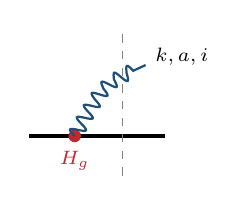
\begin{tikzpicture}[scale=0.72]
 \draw[val] (-1.2,0)--(1.2,0);
 \node[blob] at (-0.4,0) {};
 \node[acc,below] at (-0.4,-0.1) {\scriptsize $\Hg$};
 \draw[gluon] (-0.4,0) .. controls (0.1,0.9) .. (0.85,1.25);
 \node[right] at (0.85,1.4) {\scriptsize $k,a,i$};
 \draw[cut] (0.45,-0.7)--(0.45,1.9);
\end{tikzpicture}
\end{center}
\column{0.72\textwidth}
\[
\ket{\Psi^{LO}_{g\rho}}=-\int_{\Lambda}^{\vee}\!\frac{d\kp}{\sqrt{\kp}}\!\int\! d^{2}\bm k\;
\ket{g^{a}_{i}(k)}\;\frac{g\,k_{i}}{2\pi^{3/2}\bm k^{2}}\rho^{a}(-\bm k)
\]
{\small $=$ the Weizs\"acker--Williams field. Matching to $\Om\ket0$:}
\[
\mathcal{A}^{b}_{j}(p)=-\frac{\sqrt2\,g\,p_{j}\rho^{b}(-\bm p)}{\sqrt{\pp}\,\bm p^{2}}
\]
\end{columns}
\medskip
\begin{alertblock}{And the normalisation --- where the small-$x$ log lives}
\[
N=1-\frac{g^{2}}{8\pi^{3}}\int_{\Lambda}^{\vee}\!\frac{d\pp}{\pp}\!\int\! d^{2}\bm p\,\frac{\rho^{a}(-\bm p)\rho^{a}(\bm p)}{\bm p^{2}}
=1-\frac{g^{2}}{8\pi^{3}}\,\hl{\ln\frac{\vee}{\Lambda}}\int\! d^{2}\bm p\,\frac{\rho^{a}(-\bm p)\rho^{a}(\bm p)}{\bm p^{2}}
\]
The $\ln(\vee/\Lambda)=\Delta y$ is precisely the \hb{rapidity logarithm} resummed by
BFKL/JIMWLK. $\Om$ is the boost; iterating it generates the evolution equation.
\end{alertblock}
\end{frame}

%=====================================================================
\begin{frame}{Step 4 (cont.): $\mathcal{O}(g^2)$, two outgoing gluons}
Three topologies, distinguished by how many $\rho$'s they carry:
\begin{center}
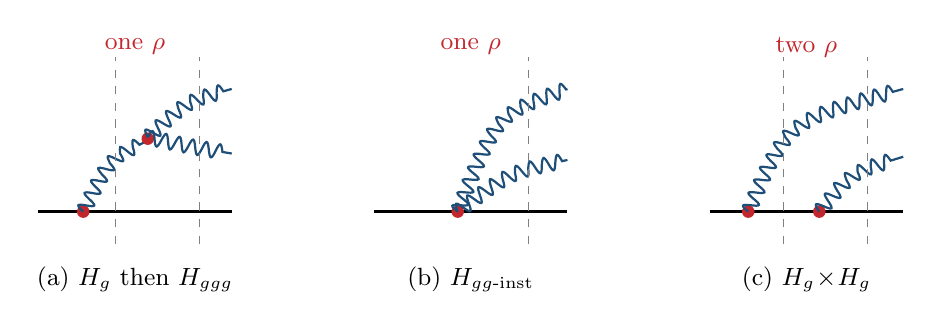
\begin{tikzpicture}[scale=0.82]
 % (a) emission + splitting
 \begin{scope}[xshift=-5.2cm]
  \draw[val] (-1.5,0)--(1.5,0);
  \node[blob] at (-0.8,0) {};
  \draw[gluon] (-0.8,0) .. controls (-0.4,0.8) .. (0.2,1.1);
  \node[blob] at (0.2,1.13) {};
  \draw[gluon] (0.2,1.15) .. controls (0.8,1.7) .. (1.5,1.9);
  \draw[gluon] (0.2,1.15) .. controls (0.9,1.0) .. (1.5,0.9);
  \draw[cut] (-0.3,-0.5)--(-0.3,2.4);
  \draw[cut] ( 1.0,-0.5)--( 1.0,2.4);
  \node[below] at (0,-0.7) {\small (a) $\Hg$ then $\Hggg$};
  \node[acc] at (0,2.55) {\small one $\rho$};
 \end{scope}
 % (b) instantaneous
 \begin{scope}[xshift=0cm]
  \draw[val] (-1.5,0)--(1.5,0);
  \node[blob] at (-0.2,0) {};
  \draw[gluon] (-0.2,0) .. controls (0.4,1.5) .. (1.5,1.9);
  \draw[gluon] (-0.2,0) .. controls (0.6,0.6) .. (1.5,0.8);
  \draw[cut] (0.9,-0.5)--(0.9,2.4);
  \node[below] at (0,-0.7) {\small (b) $H_{gg\text{-inst}}$};
  \node[acc] at (0,2.55) {\small one $\rho$};
 \end{scope}
 % (c) two independent emissions
 \begin{scope}[xshift=5.2cm]
  \draw[val] (-1.5,0)--(1.5,0);
  \node[blob] at (-0.9,0) {};
  \node[blob] at (0.2,0) {};
  \draw[gluon] (-0.9,0) .. controls (-0.3,1.4) .. (1.5,1.9);
  \draw[gluon] (0.2,0) .. controls (0.7,0.6) .. (1.5,0.85);
  \draw[cut] (-0.35,-0.5)--(-0.35,2.4);
  \draw[cut] (0.95,-0.5)--(0.95,2.4);
  \node[below] at (0,-0.7) {\small (c) $\Hg\!\times\!\Hg$};
  \node[acc] at (0,2.55) {\small two $\rho$};
 \end{scope}
\end{tikzpicture}
\end{center}
\vspace{2pt}
\begin{block}{The decomposition procedure}
\vspace{-8pt}
\[
\text{(c) gives }\rho^{b}\rho^{a}
=\tfrac12\underbrace{[\rho^{b},\rho^{a}]}_{=\,\frac{i}{2}f^{bad}\rho^{d}(-\bm k)\;\Rightarrow\;\hl{one}\ \rho}
+\;\tfrac12\underbrace{\{\rho^{b},\rho^{a}\}}_{\hl{two}\ \rho}
\]
\vspace{-2pt}
{\small The commutator part $=$ two emitters at the \emph{same} transverse point; colour algebra
collapses it to a single effective source. The anticommutator is the genuine \hb{two-source}
piece --- this makes the $\rho$-counting unambiguous.}
\end{block}
\end{frame}

%=====================================================================
\begin{frame}{Results I: the $\mathcal{O}(g)$ coefficients}
\begin{block}{Emission amplitude (one $\rho$)}
\[
\mathcal{A}^{b}_{j}(p)=-\frac{\sqrt{2}\,g\,p_{j}\,\rho^{b}(-\bm p)}{\sqrt{\pp}\,\bm p^{2}},
\qquad
N=1-g^{2}\!\int\!\dthree{p}\frac{\rho^{b}(-\bm p)\rho^{b}(\bm p)}{\pp\,\bm p^{2}}
\]
\end{block}
\begin{block}{Splitting amplitude $\ad\ad a$ --- \hl{pure $3g$ vertex, no $\rho$}}
\[
C^{cba}_{kji}(k,p,q)=\frac{i g f^{abc}\,(2\pi)^{9/2}\,\delta^{(3)}(k-p-q)}
{8\pi^{3/2}\sqrt{\kp \pp q^{+}}\Big(\frac{\bm k^{2}}{\kp}-\frac{\bm p^{2}}{\pp}-\frac{\bm q^{2}}{q^{+}}\Big)}
\Big[\cdots\text{Lipatov-like vertex}\cdots\Big]
\]
\[
[\cdots]=\Big(p_{i}-q_{i}+\tfrac{q^{+}-\pp}{\kp}k_{i}\Big)\delta_{jk}
+\Big(k_{j}+q_{j}-\tfrac{\kp+q^{+}}{\pp}p_{j}\Big)\delta_{ik}
+\Big(\tfrac{\kp+\pp}{q^{+}}q_{k}-p_{k}-k_{k}\Big)\delta_{ij}
\]
\end{block}
\medskip
\begin{itemize}
  \item $\mathcal{A}$ is the classical WW field --- one power of $\rho$, \hl{$\propto 1/g$ when $\rho\sim1/g$}.
  \item $C$ carries \hb{no} $\rho$: it is the soft gluon splitting \emph{in vacuum},
        i.e.\ the seed of the non-linear, non-Abelian structure.
  \item \hl{Both are needed at $\mathcal{O}(g)$} --- the coherent operator alone is incomplete.
\end{itemize}
\end{frame}

%=====================================================================
\begin{frame}{Results II: the $\mathcal{O}(g^{2})$ coefficients}
All of $B_{2},B_{3},D_{1},D_{2},E_{1},E_{2}$ are obtained in closed form. Structurally:
\vspace{-2pt}
\begin{block}{Two-gluon emission $B_{2}$ ($\ad\ad$)}
\hb{two independent WW emissions} $+$ \hb{WW emission then $3g$ splitting} $+$
\hb{instantaneous pair creation off $\rho$}.
\end{block}
\begin{block}{Gluon-number preserving $B_{3}$ ($\ad a$)}
The \hl{instantaneous} valence--gluon exchange with its $\Theta$-function kinematic window,
the $\{\rho,\rho\}$ Weizs\"acker--Williams piece, and the $\Hggg$ loop.
\end{block}
\begin{block}{Higher coefficients: \hl{irreducible vertex $+$ products of lower coefficients}}
\vspace{-14pt}
\begin{align*}
D_{1}&=\underbrace{\frac{[\text{4-gluon vertex}]}{E_{k}-E_{pqr}}}_{\text{irreducible}}
\;+\;\underbrace{\frac{C\,\mathcal{A}}{(\cdots)}+\frac{\mathcal{A}\,C}{(\cdots)}
+\int_{v}\frac{C\,C}{(\cdots)}}_{\text{reducible}},
\qquad
D_{2}=\frac{[\text{4-gluon}]}{(\cdots)}
+\int_{r'}\frac{C\,C^{\dagger}}{(\cdots)}
+\frac{C\mathcal{A}^{\dagger}+\mathcal{A}^{\dagger}C}{(\cdots)}\\[2pt]
E_{1}&=\frac{C\,C}{(\cdots)},\qquad E_{2}=\frac{C\,C^{\dagger}}{(\cdots)}
\qquad\Longrightarrow\qquad
\text{\normalsize the six-operator structures are \hl{entirely reducible}.}
\end{align*}
\vspace{-16pt}
\end{block}
\end{frame}

%=====================================================================
\begin{frame}{Resumming: the generator $G$}
Exponentiate to expose the connected content:
\[
\boxed{\;\Om=\exp(iG),\qquad G=G^{\dagger}\;}
\]
\small
\begin{align*}
G=&-i\int_{p}\big[\mathcal{A}\,\ad-\mathcal{A}^{\dagger}a\big]
-\tfrac{i}{2}\!\int_{p,q}\big[B_{1}-B_{2}^{\dagger}\big]aa
-\tfrac{i}{2}\!\int_{p,q}\big[B_{2}-B_{1}^{\dagger}\big]\ad\ad
-\tfrac{i}{2}\!\int_{p,q}\big[B_{3}-B_{3}^{\dagger}\big]\ad a\\
&-i\!\int_{p,q,r}\big[C\,\ad\ad a-C^{\dagger}\ad a a\big]
-\tfrac{i}{2}\!\int\big[D_{1}-D_{3}^{\dagger}\big]\ad\ad\ad a
-\tfrac{i}{2}\!\int\big[D_{2}-D_{2}^{\dagger}\big]\ad\ad a a+\cdots
\end{align*}
\normalsize
\medskip
\begin{itemize}
  \item $G$ is the \hl{generator of the infinitesimal light-cone boost}; $\Om=e^{iG}$
        promotes it to a finite boost, resumming repeated emissions and virtual corrections.
  \item Hermiticity of $G$ is automatic once the unitarity constraints are imposed ---
        a strong \hb{cross-check} on the whole calculation.
  \item $\mathcal{A},C$ enter at $\mathcal{O}(g)$; $B,D,E$ at $\mathcal{O}(g^{2})$;
        $B_{1},D_{3},E_{3}$ are fixed purely by unitarity.
\end{itemize}
\end{frame}

%=====================================================================
\begin{frame}{Application: diagonalising the soft Hamiltonian at $\mathcal{O}(g)$}
Take $H_{1}=H_{0}+\Hg+\Hggg$ and compute $\Om^{\dagger}H_{1}\Om$:
\[
\Om^{\dagger}H_{1}\Om = H_{0}+\Hg+\Hggg
+\int_{p}\Big[-\mathcal{A}\tfrac{\bm p^{2}}{2\pp}\ad+\mathcal{A}^{\dagger}\tfrac{\bm p^{2}}{2\pp}a\Big]
+\int_{p,q,r}\Big[C\big(\tfrac{\bm r^2}{2r^+}+\tfrac{\bm q^2}{2q^+}-\tfrac{\bm p^2}{2\pp}\big)\ad\ad a
- C^{\dagger}(\cdots)\ad a a\Big]
\]
Insert the explicit $\Hg,\Hggg,\mathcal{A},C$: \hl{every off-diagonal piece cancels identically}.
\[
\boxed{\;\Om^{\dagger}H_{1}\,\Om=H_{0}\;}
\]
\medskip
\begin{alertblock}{The point}
Earlier treatments diagonalised with the \hb{coherent operator $C_{\rm coh}$ alone}
(the WW field). That is \hl{not sufficient}: the non-Abelian $3g$ vertex generates an
off-diagonal structure at the \emph{same} order, and one needs the $\ad\ad a$ operator
$C$ as well. With both, the diagonalisation at $\mathcal{O}(g)$ is \hl{exact}.
\end{alertblock}
\end{frame}

%=====================================================================
\begin{frame}{Diagonalisation at $\mathcal{O}(g^{2})$}
Now keep everything: $H=H_{0}+\Hg+\Hggg+H_{gggg}+H_{gg\text{-inst}}+H_{gggg\text{-inst}}$.
\[
\Om^{\dagger}H\Om = H_{0}
\;\hb{-\int_{p}\mathcal{A}^{\dagger b}_{j}(p)\mathcal{A}^{b}_{j}(p)\frac{\bm p^{2}}{2\pp}}
\;\hg{+\,2\!\int_{p,q,r,s}\Big(\tfrac{\bm r^{2}}{2r^{+}}+\tfrac{\bm s^{2}}{2s^{+}}-\tfrac{\bm p^{2}}{2\pp}\Big)C^{\dagger}C\;\ad a}
\]
\medskip
\begin{itemize}
  \item \hg{The $C^{\dagger}C$ term vanishes identically} --- explicit evaluation gives $0$.
        No residual off-diagonal (or $\ad a$) contribution from the three-gluon sector.
  \item \hb{The coherent term survives}:
  \[
  \int\!\dthree{p}\,\mathcal{A}^{\dagger}\mathcal{A}\,\frac{\bm p^{2}}{2\pp}
  =\int\!\dthree{p}\,\frac{g^{2}\rho^{b}(\bm p)\rho^{b}(-\bm p)}{(\pp)^{2}}
  \]
\end{itemize}
\medskip
\begin{alertblock}{Final result}
\[
\boxed{\;\Om^{\dagger}H\,\Om \;=\; H_{0}\;-\;\int\!\dthree{p}\;\frac{g^{2}\,\rho^{b}(\bm p)\rho^{b}(-\bm p)}{(\pp)^{2}}\;}
\]
The only correction through $\mathcal{O}(g^{2})$ is the \hl{classical Weizs\"acker--Williams
background-field energy $\propto\rho^{2}$} --- exactly what one expects for a hadron
dressed by its own coherent gluon cloud.
\end{alertblock}
\end{frame}

%=====================================================================
\begin{frame}{What was actually new here}
\begin{columns}[T,onlytextwidth]
\column{0.5\textwidth}
\textbf{Technical}
\begin{itemize}
  \item All coefficients of the normal-ordered $\Om$ through $\mathcal{O}(g^{2})$
        in pure YM --- completing partial $\mathcal{O}(g^{2})$ results of Lublinsky--Mulian '17.
  \item Consistent treatment of \hl{operator-valued, non-commuting} $\rho$
        throughout (no classical-source shortcut).
  \item Perturbation theory reformulated for \hl{non-commuting matrix elements};
        the $[\rho,\rho]/\{\rho,\rho\}$ decomposition as a systematic $\rho$-counting.
\end{itemize}
\column{0.5\textwidth}
\textbf{Conceptual}
\begin{itemize}
  \item $\Om$ has a \hl{dual role}: it generates the LCWF \emph{and} diagonalises $H$.
  \item $\mathcal{O}(g)$ diagonalisation needs \hb{both} the coherent (WW) operator
        \emph{and} the $3g$ operator $C$.
  \item At $\mathcal{O}(g^{2})$ only the $\rho^{2}$ background energy survives ---
        a non-trivial consistency statement.
  \item Beyond LO, $\Om$ contains \hl{connected} multi-gluon amplitudes at fixed $\rho$.
\end{itemize}
\end{columns}
\vspace{-4pt}
\begin{block}{Where it goes next}
\vspace{-2pt}
{\small \hl{Single inclusive gluon production at NLO} at mid-rapidity (also needs some
$\mathcal{O}(g^{3})$ coefficients from LM~'17) \;$\bullet$\; moments of the gluon
\hb{multiplicity operator} and number \hb{fluctuations} at $\mathcal{O}(g^{4})$
\;$\bullet$\; double / triple inclusive production and the near-side ridge beyond the
coherent state.}
\end{block}
\end{frame}

%=====================================================================
\begin{frame}[standout]
Summary
\end{frame}

\begin{frame}{Take home}
\begin{enumerate}
  \item \textbf{LCPT} is ordinary time-ordered perturbation theory on null planes.
        Positivity of $\pp$ makes the vacuum trivial, so the \hl{Fock expansion of a
        hadron is a physical object}, and longitudinal boosts are kinematical.
        Cost: $A^{+}=0$ gauge brings \hb{instantaneous $1/\partial^{+}$ vertices}.
  \medskip
  \item \textbf{In the CGC}, boosting a hadron by $\Delta y$ is a \hl{unitary operator $\Om$}
        acting on the soft Fock space, with coefficients that are functionals of the
        \hb{operator-valued} valence charge density $\rho$. At LO $\Om$ is a coherent
        state of Weizs\"acker--Williams gluons.
  \medskip
  \item \textbf{This work} fixes \hl{all} coefficients of $\Om$ through $\mathcal{O}(g^{2})$
        by combining \hb{unitarity} $\Om^{\dagger}\Om=1$ with \hb{matching to LCPT}
        on $\ket0,\ket g,\ket{gg},\ket{ggg}$.
  \medskip
  \item \textbf{Check \& payoff}: $\Om^{\dagger}H\Om=H_{0}-\int g^{2}\rho\rho/(\pp)^{2}$ ---
        the Hamiltonian is diagonal up to the classical background energy. The same
        coefficients are the input for \hl{NLO gluon production, multiplicity fluctuations
        and the ridge}.
\end{enumerate}
\vfill
\begin{center}\hl{\large Thank you --- questions?}\end{center}
\end{frame}

%=====================================================================
\appendix
%=====================================================================
\begin{frame}[standout]
Backup
\end{frame}

\begin{frame}{Backup: LCPT matrix elements used}
\small
\begin{align*}
\bra{g^{a}_{i}(k)}\Hg\ket{0}&=\frac{g k_{i}\rho^{a}(-\bm k)}{4\pi^{3/2}|\kp|^{3/2}}\\[4pt]
\bk{g^{c}_{l}(q)g^{b}_{j}(p)}{\Hg\,g^{a}_{i}(k)}&=
\delta^{ac}\delta_{il}\delta^{(3)}(k-q)\frac{g p_{j}\rho^{b}(-\bm p)}{4\pi^{3/2}|\pp|^{3/2}}
+\big(p\!\leftrightarrow\!q,\,b\!\leftrightarrow\!c\big)\\[4pt]
\bk{g^{c}_{l}(q)g^{b}_{j}(p)}{\Hggg\, g^{a}_{i}(k)}&=
\frac{igf^{abc}\delta^{(3)}(k-p-q)}{8\pi^{3/2}\sqrt{\kp\pp q^{+}}}\Big[
\big(p_{i}-q_{i}+\tfrac{q^{+}-\pp}{\kp}k_{i}\big)\delta_{jl}\\
&\hspace{3.2cm}+\big(k_{j}+q_{j}-\tfrac{\kp+q^{+}}{\pp}p_{j}\big)\delta_{il}
+\big(\tfrac{\kp+\pp}{q^{+}}q_{l}-p_{l}-k_{l}\big)\delta_{ij}\Big]\\[4pt]
\bk{g^{c}_{j}(q)g^{b}_{i}(p)}{H_{gg\text{-inst}}\,0}&=
\frac{ig^{2}f^{abc}(q^{+}-\pp)\delta_{ij}\rho^{a}(-\bm p-\bm q)}{2(2\pi)^{3}\sqrt{\pp q^{+}}(\pp+q^{+})^{2}}\\[4pt]
\bk{g^{c}_{j}(q)}{H_{gg\text{-inst}}\,g^{b}_{i}(p)}&=
\frac{ig^{2}f^{abc}(\pp+q^{+})\delta_{ij}\rho^{a}(\bm p-\bm q)}{2(2\pi)^{3}\sqrt{\pp q^{+}}(\pp-q^{+})^{2}}
\end{align*}
\end{frame}

\begin{frame}{Backup: the kinematic window for $\ad a$ transitions}
\begin{columns}[T,onlytextwidth]
\column{0.45\textwidth}
For gluon-number preserving transitions off the valence background, \emph{all three}
longitudinal momenta must sit in the soft window:
\[
\Lambda<\kp<\vee,\quad \Lambda<\pp<\vee,
\]
\[
\Lambda<|\pp-\kp|<\vee .
\]
This produces the $\Theta$-functions in $B_{3}$:
\[
\Theta(\pp-\kp-\Lambda)+\Theta(\kp-\Lambda-\pp).
\]
\column{0.53\textwidth}
\vspace{-8pt}
\begin{center}
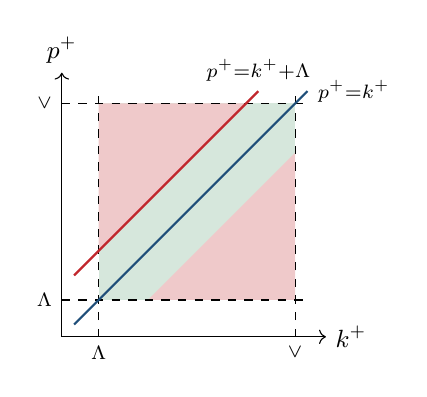
\begin{tikzpicture}[scale=0.78]
 \fill[grn!18] (0.6,0.6) rectangle (3.8,3.8);
 \fill[acc!25] (0.6,1.4) --(3.0,3.8)--(0.6,3.8)--cycle;
 \fill[acc!25] (1.4,0.6) --(3.8,3.0)--(3.8,0.6)--cycle;
 \draw[->] (0,0)--(4.3,0) node[right]{\small $\kp$};
 \draw[->] (0,0)--(0,4.3) node[above]{\small $\pp$};
 \draw[dashed] (0.6,0)--(0.6,4.0); \node[below] at (0.6,0) {\scriptsize $\Lambda$};
 \draw[dashed] (3.8,0)--(3.8,4.0); \node[below] at (3.8,0) {\scriptsize $\vee$};
 \draw[dashed] (0,0.6)--(4.0,0.6); \node[left] at (0,0.6) {\scriptsize $\Lambda$};
 \draw[dashed] (0,3.8)--(4.0,3.8); \node[left] at (0,3.8) {\scriptsize $\vee$};
 \draw[thick,blu] (0.2,0.2)--(4.0,4.0) node[right,black]{\scriptsize $\pp{=}\kp$};
 \draw[thick,acc] (0.2,1.0)--(3.2,4.0) node[above,black]{\scriptsize $\pp{=}\kp{+}\Lambda$};
\end{tikzpicture}
\end{center}
\end{columns}
\vspace{-2pt}
{\small The intersection of the shaded regions is the allowed $\pp$ range; the two
$\Theta$-functions correspond to $\pp$ above / below the incoming $\kp$, i.e.\ to longitudinal
momentum flowing out of / into the valence sector.}
\end{frame}

\begin{frame}{Backup: perturbation theory with non-commuting matrix elements}
Standard Rayleigh--Schr\"odinger, but the matrix elements are \hl{operators in the valence
Hilbert space} and must be kept in order:
\[
\ket{n}=\ket{n^{(0)}}-\sum_{i\neq0}\frac{\ket{n^{(i)}}\bra{n^{(i)}}H_{\rm int}\ket{n^{(0)}}}
{E^{(0)}_{i}-E^{(0)}_{0}-E^{(1)}_{i}-E^{(2)}_{i}}
+\sum_{i,j\neq0}\frac{\ket{n^{(i)}}\bra{n^{(i)}}H_{\rm int}\ket{n^{(j)}}\bra{n^{(j)}}H_{\rm int}\ket{n^{(0)}}}
{\big(E^{(0)}_{i}-E^{(0)}_{0}-E^{(1)}_{i}\big)\big(E^{(0)}_{j}-E^{(0)}_{0}-E^{(1)}_{j}\big)}
\]
with $E^{(1)}_{i}\equiv\bra{n^{(i)}}H_{\rm int}\ket{n^{(i)}}$.
\medskip
\begin{block}{Why it matters}
For $E_{0}^{(0)}=0$ (the soft vacuum),
\[
\ket{\psi}_{N}=\ket0-\frac{\ket{n^{(i)}}\bra{n^{(i)}}H_{\rm int}\ket{0}}{E^{(0)}_{i}}
+\frac{\ket{n^{(i)}}\bra{n^{(i)}}H_{\rm int}\ket{n^{(j)}}\bra{n^{(j)}}H_{\rm int}\ket{0}}{E^{(0)}_{i}E^{(0)}_{j}} .
\]
Writing $\bra{i}H\ket{j}\bra{j}H\ket{0}$ in the \emph{wrong} order would change the
colour structure at $\mathcal{O}(g^{2})$ --- this is the difference between
$[\rho,\rho]$ and $\{\rho,\rho\}$ contributions.
\end{block}
\end{frame}

\begin{frame}{Backup: dictionary for the equal-time--minded}
\begin{center}
\small
\begin{tabular}{p{3.0cm}p{4.6cm}p{4.0cm}}
\toprule
& \textbf{equal time} ($t=0$) & \textbf{light front} ($\xp=0$)\\
\midrule
Hamiltonian & $P^{0}$ & $P^{-}$\\
Dispersion & $E=\sqrt{\bm p^{2}+m^{2}}$ & $p^{-}=\frac{\bm p^{2}+m^{2}}{2\pp}$\\
Vacuum & non-trivial condensate & \hl{trivial} (perturbatively)\\
Boost along $z$ & dynamical & \hl{kinematical}\\
Gauge & $A^{0}=0$ (Coulomb term) & $A^{+}=0$ (inst.\ $1/\partial^{+}$)\\
Fock expansion & frame dependent & \hl{frame independent}\\
Ghosts & yes (covariant gauges) & no\\
Pathologies & --- & $\pp\to0$ zero modes\\
\bottomrule
\end{tabular}
\end{center}
\medskip
\begin{block}{The trade}
Light-front quantisation buys a probabilistic, boost-invariant description of the
hadron. It pays for it with a singular $\pp\to0$ region --- which in the small-$x$
context is not a bug: the $\ln(\vee/\Lambda)$ divergence \hl{is} the rapidity evolution.
\end{block}
\end{frame}

\end{document}
